% Provenance (never printed): see sources/outline_sources.md (Year 3:
% spectral signatures; optical, thermal and radar sensors; radar
% interferometry; digital elevation models; GIS operations).
% Brief: sources/book5/BRIEFS.md, ch. 25. Curves from figdata/bachelor-3/
% spectral_signatures.py (ECOSTRESS spectra and the Landsat 8 OLI bands),
% thermal_ir.py (Planck's law, brightness temperatures, a mixed pixel),
% insar_mogi.py (the wrapped interferogram of a Mogi source) and
% varden_gis.py (slope, aspect and an overlay on the Varden Hills, from
% figdata/shared/region.py, read only). Exercise and problem values in the
% Book 5 scratch calculator calc/ch25.py. Mount Halvren, its lava flows and
% its fumaroles are invented. The brief's overlay (slope > 15 degrees on
% limestone within 200 m of the river) is empty on the Varden model: the
% valley floor is flat; the printed overlay uses the shale within 1 km.
\chapter{Remote Sensing and GIS}\label{ch:b3:remote-sensing-gis}

In 1997 the ground of a wilderness in the Cascade Range, near the cluster of
volcanoes called the Three Sisters, began to rise. By 2001 its centre stood
\qty{15}{cm} higher. No volcano stands directly above the swelling, and the
last eruption in the area was 1,500 years old. The uplift was not found by
anyone walking on it: it appeared as a bull's eye of coloured rings when
radar images of the region, taken from orbit years apart, were combined.
The rings placed the intruding magma 6 to \qty{7}{km} down; in March 2004
a swarm of more than 300 small earthquakes struck next to their centre.
This chapter explains how a satellite measures a change of a few
centimetres from hundreds of kilometres up, what the other sensors in orbit
see of the ground, and how the maps they make are combined in a geographic
information system.
% ledger: usgs:insar-fs

\begin{recall}
The electromagnetic spectrum, Planck's law of the black body, emissivity
and Kirchhoff's law, reflectance and the interference of waves are in the
physics books. Remote sensing, satellite images, map projections and
satellite positioning are in the school books. Atmospheric windows and
photometric bands are in the Year~1 volume, in its chapter on telescopes;
the digital elevation model and the geographic information system that
stores it, in its chapter on geological maps; the first radar map of an
earthquake's displacement, in its chapter on the earthquake source. The
Mogi source of an inflating magma reservoir is in the Year~2 volume, in its
chapter on volcanic eruptions.
\end{recall}

\section{Spectral signatures and optical sensors}\label{sec:b3:remote-sensing-gis:optical}

Sunlight that reaches the ground is partly absorbed and partly reflected,
in proportions that depend on the wavelength and on what the ground is
made of. A sensor in orbit measures the reflected light in a few ranges of
wavelength, its bands, and the ratios between the bands identify the
surface.

\begin{definition}[Spectral signature]\label{def:b3:remote-sensing-gis:signature}
The \emph{spectral signature}\index{spectral signature} of a material is
its reflectance as a function of wavelength, $R(\lambda)$, the fraction of
the incident radiation it reflects. Over the thermal infrared, where
surfaces emit rather than reflect, the signature is the emissivity
$\varepsilon(\lambda)$; for an opaque sample $\varepsilon = 1 - R$.
\end{definition}

\begin{omfigure}
\centering
\begin{tikzpicture}
\begin{axis}[width=0.9\linewidth, height=6.4cm, xmin=0.4, xmax=2.5, ymin=0, ymax=1,
  xlabel={wavelength (\unit{\micro\metre})}, ylabel={reflectance},
  tick label style={font=\scriptsize}, label style={font=\small},
  legend style={font=\scriptsize, at={(0.5,-0.24)}, anchor=north, /tikz/every even column/.append style={column sep=4pt}},
  legend columns=5, clip=false]
\fill[black!8] (axis cs:0.45,0) rectangle (axis cs:0.51,1);
\fill[black!8] (axis cs:0.53,0) rectangle (axis cs:0.59,1);
\fill[black!8] (axis cs:0.64,0) rectangle (axis cs:0.67,1);
\fill[black!8] (axis cs:0.85,0) rectangle (axis cs:0.88,1);
\fill[black!8] (axis cs:1.57,0) rectangle (axis cs:1.65,1);
\fill[black!8] (axis cs:2.11,0) rectangle (axis cs:2.29,1);
\addplot[very thick, green!50!black] table[x=um, y=grass] {figdata/out/bachelor-3-spectral_signatures-spectra.dat};
\addlegendentry{green grass}
\addplot[thick, brown!70!black, dashed] table[x=um, y=soil] {figdata/out/bachelor-3-spectral_signatures-spectra.dat};
\addlegendentry{brown sand soil}
\addplot[thick, black!55] table[x=um, y=kaol] {figdata/out/bachelor-3-spectral_signatures-spectra.dat};
\addlegendentry{kaolinite}
\addplot[thick, red!70!black, dash dot] table[x=um, y=hem] {figdata/out/bachelor-3-spectral_signatures-spectra.dat};
\addlegendentry{haematite}
\addplot[thick, omDef] table[x=um, y=water] {figdata/out/bachelor-3-spectral_signatures-spectra.dat};
\addlegendentry{water}
\node[font=\tiny, anchor=south] at (axis cs:0.48,1) {2};
\node[font=\tiny, anchor=south] at (axis cs:0.56,1) {3};
\node[font=\tiny, anchor=south] at (axis cs:0.655,1) {4};
\node[font=\tiny, anchor=south] at (axis cs:0.865,1) {5};
\node[font=\tiny, anchor=south] at (axis cs:1.61,1) {6};
\node[font=\tiny, anchor=south] at (axis cs:2.2,1) {7};
\end{axis}
\end{tikzpicture}
\par\smallskip{\small Laboratory reflectance spectra of five surfaces (ECOSTRESS
Spectral Library, reproduced through the courtesy of the Jet Propulsion
Laboratory, California Institute of Technology), with the six reflective
bands 2 to 7 of the Landsat~8 and 9 imager shaded. Green grass is dark in
the visible, brightest in the near infrared; kaolinite is bright everywhere
but for a narrow absorption at \qty{2.2}{\micro\metre}; haematite absorbs
the blue and green and reflects the red; water reflects a few percent at
every wavelength.}\label{fig:b3:remote-sensing-gis:spectra}
\end{omfigure}
% ledger: data:b5-ecostress, usgs:landsat8-bands, nasa:ndvi

The signatures in the figure above are the vocabulary of optical remote
sensing. The chlorophyll of leaves absorbs strongly between 0.4 and
\qty{0.7}{\micro\metre}, for photosynthesis, while the cells of the leaves
reflect strongly between 0.7 and \qty{1.1}{\micro\metre}: green grass
reflects \qty{5}{\percent} of the red light of band~4 and \qty{50}{\percent}
of the near infrared of band~5, a jump no rock or soil makes. Beyond, two
deep dips near 1.4 and \qty{1.9}{\micro\metre} are where liquid water
absorbs. The brown sand brightens steadily towards the infrared. Kaolinite,
a clay, is white in the visible and has a narrow absorption at
\qty{2.20}{\micro\metre}, inside band~7, which makes it darker there than
in band~6; a \omterm{def:b3:remote-sensing-gis:sensors}{hyperspectral sensor} resolves its shape and tells one clay from
another. Haematite absorbs the blue and green: hence its red.
% ledger: nasa:ndvi, data:b5-ecostress

\begin{definition}[Spatial, spectral and radiometric resolution; revisit time]\label{def:b3:remote-sensing-gis:resolutions}
The \emph{spatial resolution}\index{spatial resolution} of an image is the
size on the ground of one of its pixels. Its \emph{spectral
resolution}\index{spectral resolution} is the number and width of its
bands, its \emph{radiometric resolution}\index{radiometric resolution} the
number of levels in which each measurement is recorded, $2^b$ for $b$ bits.
The \emph{revisit time}\index{revisit time} of a satellite is the interval
between two of its observations of the same place.
\end{definition}

The four cannot all be fine at once: smaller pixels and narrower bands
collect less light each, and a narrow swath takes longer to cover the
Earth. The imager of Landsat~8, launched in 2013, has nine bands, most of
them with \qty{30}{m} pixels and one panchromatic band at \qty{15}{m}; it
records 4096 levels (12 bits) where the instruments of Landsats 1 to 7
recorded 256. From a sun-synchronous orbit \qty{705}{km} up it images a
swath \qty{185}{km} wide and returns over the same ground every 16 days;
Landsat~9, in the same orbit 8 days apart, halves the wait. The
multispectral imager of each Sentinel-2 satellite has 13 bands, at 10, 20
or \qty{60}{m}, over a swath of \qty{290}{km}; with two satellites in the
same orbit the revisit at the Equator is 5 days.
% ledger: usgs:landsat8-bands, usgs:landsat8-orbit, esa:s2-msi, esa:s2-orbit

\begin{definition}[Multispectral and hyperspectral sensors]\label{def:b3:remote-sensing-gis:sensors}
A \emph{multispectral sensor}\index{multispectral sensor} records a few
to a few tens of bands, separated by gaps. A \emph{hyperspectral
sensor}\index{hyperspectral sensor} records many narrow, contiguous bands,
so that every pixel carries a nearly continuous spectrum that can be
compared with a library such as the one of the figure above.
\end{definition}

Between the ground and the sensor lies the atmosphere. It scatters
sunlight into the sensor that never touched the ground, most of all at
short wavelengths, the path radiance, and it absorbs part of what the
ground reflects outside the windows.

\begin{definition}[Atmospheric correction]\label{def:b3:remote-sensing-gis:atm-correction}
\emph{Atmospheric correction}\index{atmospheric correction} is the
conversion of the radiance measured at the top of the atmosphere into the
reflectance of the surface, by removing the path radiance and compensating
the absorption along the two paths of the light, down and up.
\end{definition}

The simplest correction subtracts in each band the value of the darkest
pixels of the scene, deep clear water or a shadow, which should reflect
nearly nothing: what they show is the path radiance. Careful corrections
model the atmosphere's molecules, aerosols and water vapour.

\begin{definition}[Normalised difference vegetation index]\label{def:b3:remote-sensing-gis:ndvi}
The \emph{normalised difference vegetation
index}\index{normalised difference vegetation index} (NDVI) of a pixel is
\[
\mathrm{NDVI} = \frac{R_\mathrm{NIR} - R_\mathrm{red}}{R_\mathrm{NIR} + R_\mathrm{red}} ,
\]
computed from its reflectances in a near-infrared and a red band.
\end{definition}

The index lies between $-1$ and $+1$. Ground without green leaves gives a
value close to zero, barren rock, sand or snow \num{0.1} and below,
shrubs and grassland 0.2 to 0.3, temperate and tropical rainforests 0.6 to
0.8; the densest green leaves approach 0.8 to 0.9. From the spectra of the
figure above, through bands 4 and 5, the grass gives 0.82, the brown sand
0.15 and the water $-0.01$. Being a ratio, the index does not change when
both bands are dimmed in the same proportion, by a slope facing away from
the light or a thin uniform haze: it measures the vegetation, not the
illumination. An additive path radiance, larger in the red, does change it,
which is why the index is computed from corrected reflectances
(\cref{exo:b3:remote-sensing-gis:12}).
% ledger: nasa:ndvi, data:b5-ecostress

\section{The thermal infrared}\label{sec:b3:remote-sensing-gis:thermal}

At the temperatures of the ground, around \qty{300}{K}, Planck's law puts
the peak of a black body's emission near \qty{9.7}{\micro\metre}, in the
atmospheric window of the thermal infrared. There the sensor measures what
the surface emits, not what it reflects. The thermal sensor of Landsat~8
has two bands, 10.6 to 11.19 and 11.5 to \qty{12.51}{\micro\metre}, with
\qty{100}{m} pixels.
% ledger: const:h, const:c, const:kB, usgs:landsat8-bands

\begin{definition}[Brightness temperature]\label{def:b3:remote-sensing-gis:brightness}
The \emph{brightness temperature}\index{brightness temperature} $T_b$ of a
surface at the wavelength $\lambda$ is the temperature of the black body
that would emit the spectral radiance $L$ measured from it at that
wavelength. The \emph{kinetic temperature} is the surface's thermodynamic
temperature, the one a thermometer would read.
\end{definition}

\begin{proposition}[Brightness temperature from a radiance]\label{prop:b3:remote-sensing-gis:planck-inversion}
With $c_1 = 2hc^2$ and $c_2 = hc/k$, a spectral radiance $L$ at the
wavelength $\lambda$ has the \omterm{def:b3:remote-sensing-gis:brightness}{brightness temperature}
\[
T_b = \frac{c_2}{\lambda \ln\!\left(1 + \dfrac{c_1}{\lambda^5 L}\right)} .
\]
A surface of emissivity $\varepsilon < 1$ at the kinetic temperature $T$
emits $L = \varepsilon B_\lambda(T)$ and has $T_b < T$.
\end{proposition}

\begin{proof}
Planck's law gives $B_\lambda(T) = c_1\lambda^{-5}/(e^{c_2/\lambda T} -
1)$. Setting $B_\lambda(T_b) = L$ and solving, $e^{c_2/\lambda T_b} = 1 +
c_1/(\lambda^5L)$, which is the formula. $B_\lambda$ increases with the
temperature, so $\varepsilon B_\lambda(T) < B_\lambda(T)$ implies $T_b < T$.
\end{proof}
% ledger: const:h, const:c, const:kB

The difference matters. At the centre of band~10, \qty{10.9}{\micro\metre},
a surface at \qty{300}{K} with an emissivity of 0.95 has a \omterm{def:b3:remote-sensing-gis:brightness}{brightness
temperature} of \qty{296.6}{K}, one of 0.99 \qty{299.3}{K}: a percent of
emissivity is worth more than half a kelvin. The laboratory spectra give,
in band~10, an emissivity of 0.98 for the grass, 0.99 for the water and
0.97 for the brown sand. Mapping a temperature from orbit therefore needs
the emissivity of every pixel, and a correction for the emission and the
absorption of the air between.
% ledger: data:b5-ecostress

\begin{omfigure}
\centering
\begin{tikzpicture}
\begin{groupplot}[group style={group size=2 by 1, horizontal sep=1.5cm},
  width=0.48\linewidth, height=0.42\linewidth,
  tick label style={font=\scriptsize}, label style={font=\small}, title style={font=\small}]
\nextgroupplot[title={black-body radiance}, xmode=log, ymode=log, xmin=1, xmax=25,
  ymin=0.01, ymax=1e5, xlabel={wavelength (\unit{\micro\metre})},
  ylabel={$B_\lambda$ (\unit{W.m^{-2}.sr^{-1}.\micro\metre^{-1}})},
  xtick={1,2,5,10,20}, xticklabels={1,2,5,10,20}]
\fill[black!10] (axis cs:10.6,0.01) rectangle (axis cs:11.19,1e5);
\fill[black!10] (axis cs:2.11,0.01) rectangle (axis cs:2.29,1e5);
\addplot[thick, omDef] table[x=um, y=b300] {figdata/out/bachelor-3-thermal_ir-planck.dat};
\addplot[thick, omDef, dashed] table[x=um, y=b400] {figdata/out/bachelor-3-thermal_ir-planck.dat};
\addplot[thick, red!70!black] table[x=um, y=b1443] {figdata/out/bachelor-3-thermal_ir-planck.dat};
\node[font=\scriptsize, omDef, anchor=north east] at (axis cs:24,3) {\qty{300}{K}};
\node[font=\scriptsize, omDef, anchor=south west] at (axis cs:12.5,30) {\qty{400}{K}};
\node[font=\scriptsize, red!70!black, anchor=south west] at (axis cs:3.2,2000) {\qty{1443}{K}};
\node[font=\tiny, anchor=north] at (axis cs:10.9,1e5) {10};
\node[font=\tiny, anchor=north] at (axis cs:2.2,1e5) {7};
\nextgroupplot[title={a mixed pixel, band 10}, xmin=0, xmax=1, ymin=285, ymax=375,
  xlabel={fraction $f$ of the pixel at \qty{370}{K}}, ylabel={temperature (\unit{K})},
  legend style={font=\scriptsize, at={(0.97,0.03)}, anchor=south east}]
\addplot[thick, red!70!black] table[x=f, y=tb] {figdata/out/bachelor-3-thermal_ir-mixed.dat};
\addlegendentry{brightness temperature}
\addplot[thick, black!60, dashed, domain=0:1] {290 + 80*x};
\addlegendentry{mean temperature}
\end{groupplot}
\end{tikzpicture}
\par\smallskip{\small Left, Planck's law for surfaces at 300 and \qty{400}{K}
and for the lava of an eruption at \qty{1170}{\celsius} (\qty{1443}{K}), with
the shortwave infrared band~7 and the thermal band~10 of Landsat~8 shaded.
Right, the \omterm{def:b3:remote-sensing-gis:brightness}{brightness temperature} in band~10 of a pixel in which a fraction
$f$ is at \qty{370}{K} and the rest at \qty{290}{K}, against the
area-weighted mean temperature: the hot part counts for more than its
area.}\label{fig:b3:remote-sensing-gis:thermal}
\end{omfigure}
% ledger: const:h, const:c, const:kB, usgs:landsat8-bands, usgs:kilauea-temp

Lava at \qty{1170}{\celsius} has its peak near \qty{2.0}{\micro\metre}: a
fresh lava flow far smaller than a pixel lights up the shortwave infrared
bands of an optical imager, by day or night. A pixel is rarely uniform, and
Planck's law is not linear in the temperature.
% ledger: usgs:kilauea-temp

\begin{proposition}[A mixed pixel]\label{prop:b3:remote-sensing-gis:mixed}
A pixel of which a fraction $f$ emits as a black body at $T_h$ and the rest
at $T_0 < T_h$ has the radiance $L = fB_\lambda(T_h) + (1 - f)B_\lambda(T_0)$,
and, for $0 < f < 1$, its \omterm{def:b3:remote-sensing-gis:brightness}{brightness temperature} exceeds the area-weighted
mean temperature $fT_h + (1 - f)T_0$.
\end{proposition}

\begin{proof}
The radiance is the area-weighted mean of the radiances. Write $B_\lambda(T)
= c_1\lambda^{-5}g(c_2/\lambda T)$ with $g(x) = 1/(e^x - 1)$; in the
variable $T$, with $x = c_2/\lambda T$, the second derivative of
$g(c_2/\lambda T)$ is $(x g''(x) + 2g'(x))\,x/T^2$, positive when $x(e^x + 1)
> 2(e^x - 1)$, that is $x > 2\tanh(x/2)$, which holds for every $x > 0$:
$B_\lambda$ is convex in $T$. By convexity
the mean of the radiances exceeds the radiance of the mean temperature, and
$B_\lambda$ increases with $T$, so $T_b > fT_h + (1 - f)T_0$.
\end{proof}

A pixel with \qty{5}{\percent} of
fumarole ground at \qty{370}{K} in a background at \qty{290}{K} has a mean
temperature of \qty{294}{K} but a \omterm{def:b3:remote-sensing-gis:brightness}{brightness temperature} of \qty{295.3}{K};
at \qty{10}{\percent}, \qty{300.4}{K}. Hot spots stand out of a thermal
image, and their temperature cannot be read from one band alone: two bands
of different wavelength give two equations for $f$ and $T_h$.

\section{Radar and lidar}\label{sec:b3:remote-sensing-gis:radar}

An optical or thermal sensor is passive: it measures the light the ground
sends. A radar or a \omterm{def:b3:remote-sensing-gis:lidar}{lidar} is active: it sends a pulse and times its echo.
Microwaves pass through clouds, and the radar brings its own illumination,
so it observes by day and night in any weather.
% ledger: esa:s1-sar

\begin{definition}[Synthetic-aperture radar; radar backscatter]\label{def:b3:remote-sensing-gis:sar}
A \emph{synthetic-aperture radar}\index{synthetic-aperture radar} (SAR)
is a radar carried along a track that looks sideways, and that combines the
echoes it records from the same point of the ground along a length of its
track, keeping their phases, as if they had been received by one antenna as
long as that length. The \emph{radar backscatter}\index{radar backscatter}
of a surface is the fraction of the power it receives that it sends back
towards the antenna.
\end{definition}

\begin{omfigure}
\centering
\begin{tikzpicture}[>=stealth, font=\small, x=1cm, y=1cm]
\fill[black!12] (-0.5,-0.35) rectangle (10.5,0);
\draw[thick] (-0.5,0) -- (10.5,0);
% satellite
\fill[omDef] (0.6,4.6) rectangle (1.4,5.0);
\draw[thick, omDef] (0.35,4.45) -- (1.65,5.15);
\draw (1.0,4.8) circle (0.12); \fill (1.0,4.8) circle (0.03);
\node[font=\scriptsize, anchor=south, align=center] at (1.0,5.3) {flight (azimuth)\\into the page};
% nadir
\draw[dashed, black!60] (1.0,4.4) -- (1.0,0);
\node[font=\scriptsize, anchor=north] at (1.0,-0.4) {nadir};
\draw[<->, black!60] (0.3,0) -- node[left, font=\scriptsize] {$h$} (0.3,4.4);
% beam
\fill[omDef!12] (1.0,4.4) -- (4.3,0) -- (9.6,0) -- cycle;
\draw[omDef!60] (1.0,4.4) -- (4.3,0); \draw[omDef!60] (1.0,4.4) -- (9.6,0);
\node[font=\scriptsize, anchor=north] at (4.3,-0.4) {near range};
\node[font=\scriptsize, anchor=north] at (9.6,-0.4) {far range};
\draw[<->] (4.3,-1.0) -- node[below, font=\scriptsize] {swath} (9.6,-1.0);
% target and slant range
\fill[red!70!black] (7.0,0) circle (0.07);
\draw[thick, red!70!black] (1.0,4.4) -- node[above, sloped, font=\scriptsize] {slant range $R$} (7.0,0);
\draw[black!60] (7.0,0) -- (7.0,1.8);
\draw[black!60] (7.0,0.9) arc (90:126.25:0.9);
\node[font=\scriptsize] at (6.6,1.2) {$\theta$};
\draw[->, very thick, omThm] (7.0,0) -- (6.2,0.59) node[anchor=north east, font=\scriptsize, inner sep=1pt] {LOS};
\draw[<->, black!60] (1.0,-1.6) -- node[below, font=\scriptsize] {ground range} (7.0,-1.6);
\draw[black!60] (1.0,-1.5) -- (1.0,-1.7); \draw[black!60] (7.0,-1.5) -- (7.0,-1.7);
\end{tikzpicture}
\par\smallskip{\small The geometry of a side-looking radar, in the plane
perpendicular to its track. The beam lights a swath to one side of the
nadir; a point of the ground is seen at the slant range $R$ under the
incidence angle $\theta$, along the \omterm{def:b3:remote-sensing-gis:insar}{line of sight} (LOS). Echoes are sorted
by their delay across the track, in range, and by the phase history of the
synthetic aperture along it, in azimuth.}\label{fig:b3:remote-sensing-gis:sar}
\end{omfigure}

\begin{proposition}[Azimuth resolution]\label{prop:b3:remote-sensing-gis:azimuth}
A real antenna of length $L$ at the slant range $R$ separates two points of
the ground along its track only if they are more than about $R\lambda/L$
apart. A \omterm{def:b3:remote-sensing-gis:sar}{synthetic-aperture radar} with the same antenna reaches about $L/2$,
whatever the range.
\end{proposition}

\begin{proof}
The beam of an antenna of length $L$ spreads over an angle of about
$\lambda/L$, so it lights a strip $R\lambda/L$ long along the track, and
the real antenna cannot tell apart two points inside it. A point stays in
the beam while the antenna travels that same length $\ell = R\lambda/L$:
this is the synthetic aperture. Combining the echoes over $\ell$ is
equivalent to an antenna of length $\ell$; the path of each echo is
travelled twice, out and back, which halves the beam of the synthetic
antenna to $\lambda/(2\ell)$, and the resolution is $R\lambda/(2\ell) =
L/2$. A farther point stays longer in the beam, and the longer aperture
exactly compensates the larger range.
\end{proof}

The radar of each Sentinel-1 satellite works in the C band, at
\qty{5.405}{GHz}, a wavelength of about \qty{5.55}{cm}, with an antenna
\qty{12.3}{m} long, from \qty{693}{km} up. A real antenna that size would
see details no finer than about \qty{4}{km} along the track; the synthetic
aperture brings $L/2$ to about \qty{6}{m}. Over land it works mostly in a
wide-swath mode that scans three sub-swaths to cover \qty{250}{km}, at
incidence angles between 29 and \ang{46}, with cells of 5 by \qty{20}{m}.
One satellite repeats its orbit every 12 days.
% ledger: esa:s1-sar, esa:s1-orbit, esa:s1-iw

The backscatter depends on the roughness of the surface at the scale of the
wavelength and on its moisture. A calm lake reflects the pulse away, like a
mirror, and is black; a rough lava flow, a forest canopy or a city of walls
and corners sends much of it back and is bright.

\begin{definition}[Lidar]\label{def:b3:remote-sensing-gis:lidar}
A \emph{lidar}\index{lidar} measures distances by the travel time of laser
pulses reflected by the ground, the vegetation or the water.
\end{definition}

\begin{proposition}[Time of flight]\label{prop:b3:remote-sensing-gis:tof}
A pulse that returns a time $t$ after it left has met a surface at the
distance $ct/2$; an uncertainty $\delta t$ on the time is an uncertainty
$c\,\delta t/2$ on the distance.
\end{proposition}

\begin{proof}
The light travels at $c$ out and back, the distance $2d = ct$.
\end{proof}

The laser altimeter of ICESat-2, about \qty{500}{km} up, fires
\num{10000} pulses a second at \qty{532}{nm} in six beams, one every
\qty{0.7}{m} along the ground in a footprint \qty{11}{m} across. Of the
about 300~trillion photons that leave with each pulse only about a dozen
return, and each is timed to \qty{800}{ps}: \qty{12}{cm} of range. Over a
forest some photons return from the canopy and some from the ground
through its gaps: the difference is the height of the trees, and the
ground photons alone give a map of the relief beneath. \omterm{def:b3:remote-sensing-gis:lidar}{Lidars} flown on
aircraft map the ground under the vegetation the same way.
% ledger: nasa:icesat2-atlas, nasa:icesat2-photons

\section{Radar interferometry}\label{sec:b3:remote-sensing-gis:insar}

The echo recorded by a radar has an amplitude, the strength of the return,
and a phase, which counts the round-trip distance in units of the
wavelength. The phase of one image alone is useless: each pixel holds many
scatterers whose echoes add with random phases. But if the ground does not
change in between, the same scatterers give the same sum again.
% ledger: usgs:insar-vhp

\begin{definition}[Radar interferometry; interferogram; line of sight]\label{def:b3:remote-sensing-gis:insar}
\emph{Radar interferometry}\index{radar interferometry} (InSAR) combines
two radar images of the same ground, taken from nearly the same position
at two times, pixel by pixel. Their \emph{interferogram}\index{interferogram}
is the map of the difference of their phases, known modulo $2\pi$ and
drawn as a cycle of colours, one cycle a \emph{fringe}. The \emph{line of
sight}\index{line of sight (radar)} is the direction from the ground to
the antenna; the radar measures only the component of a displacement along
it. \emph{Phase unwrapping}\index{phase unwrapping} is the reconstruction
of the continuous phase from the wrapped one, by adding to each pixel the
multiple of $2\pi$ that makes the phase vary smoothly from its neighbours.
\end{definition}

\begin{theorem}[One fringe]\label{thm:b3:remote-sensing-gis:fringe}
Between two acquisitions from the same position, a displacement of the
ground that shortens the distance to the antenna by $\Delta r$ changes the
phase of its echo by $\Delta\phi = 4\pi\Delta r/\lambda$. One fringe, a
change of $2\pi$, is a motion of $\lambda/2$ along the \omterm{def:b3:remote-sensing-gis:insar}{line of sight}.
\end{theorem}

\begin{proof}
The echo travels the distance $2r$, out and back, and its phase is
$2\pi\cdot 2r/\lambda$ plus a constant fixed by the scatterers, the same in
both images. The difference is $4\pi\Delta r/\lambda$, and it is $2\pi$
for $\Delta r = \lambda/2$.
\end{proof}

For Sentinel-1 a fringe is \qty{27.7}{mm}; for the older European and
Canadian satellites, of wavelength \qty{5.66}{cm}, \qty{28.3}{mm}, the
cycle of colours of the photograph below. In practice the positions of the
two passes differ, by up to a hundred metres or so (Sentinel-1 is held
within \qty{120}{m} of a reference orbit), and the phase difference
also contains the relief, which a digital elevation model removes; the
atmosphere's water vapour delays the waves differently on the two dates;
and where the ground changes between the passes, vegetation above all, the
phases lose their coherence and the fringes dissolve into noise. The longer
L-band wavelength, \qty{23.53}{cm}, sees through vegetation better than the
C band.
% ledger: esa:s1-sar, esa:s1-orbit, usgs:insar-fs, photo:b3-three-sisters-insar

\begin{proposition}[A Mogi source seen along the line of sight]\label{prop:b3:remote-sensing-gis:mogi-los}
Above a Mogi source of volume change $\Delta V$ at depth $z_0$, at the
horizontal distance $r$, the ground moves up by $u_z$, as in the Year~2
volume, and outwards by
\[
u_r = \frac{(1 - \nu)\,\Delta V}{\pi}\,\frac{r}{(r^2 + z_0^2)^{3/2}} = \frac{r}{z_0}\,u_z .
\]
Seen at the incidence $\theta$ from a satellite to the east, the change of
the \omterm{def:b3:remote-sensing-gis:insar}{line of sight} is $d = u_E\sin\theta + u_z\cos\theta$, $u_E$ the
eastward displacement. Along the north--south line through the centre,
$d = u_z\cos\theta$.
\end{proposition}

\begin{proof}
The radial formula is the companion of the vertical one in the same
solution. The unit vector from the ground to the satellite is
$(\sin\theta, 0, \cos\theta)$ in east, north and up, and the change of the
distance is minus the projection of the displacement on it, so the
shortening is $d$. On the north--south line the outward motion is
northward or southward, perpendicular to that vector, and $u_E = 0$.
\end{proof}
% ledger: dmodels:mogi, dmodels:mogi-radial

\begin{omfigure}
\centering
\begin{tikzpicture}
\begin{groupplot}[group style={group size=2 by 1, horizontal sep=1.5cm},
  tick label style={font=\scriptsize}, label style={font=\small}, title style={font=\small}]
\nextgroupplot[title={wrapped interferogram}, width=0.46\linewidth, height=0.46\linewidth,
  axis equal image, enlargelimits=false, xmin=-15, xmax=15, ymin=-15, ymax=15,
  xlabel={east (km)}, ylabel={north (km)},
  colormap={fringe}{rgb255=(128,0,170) rgb255=(30,60,220) rgb255=(0,170,220) rgb255=(30,170,60) rgb255=(240,220,0) rgb255=(240,120,0) rgb255=(220,20,30) rgb255=(128,0,170)},
  point meta min=0, point meta max=6.2832]
\addplot[matrix plot*, mesh/cols=101, point meta=explicit] table[x=x, y=y, meta=phase] {figdata/out/bachelor-3-insar_mogi-map.dat};
\draw[->, very thick, white] (axis cs:6,-12.5) -- (axis cs:12,-12.5);
\node[font=\scriptsize, white, anchor=south] at (axis cs:9,-12.3) {to satellite};
\nextgroupplot[title={profiles}, width=0.5\linewidth, height=0.46\linewidth,
  xmin=-15, xmax=15, ymin=-60, ymax=240, xlabel={distance from the centre (km)},
  ylabel={displacement (\unit{mm})}, legend columns=2,
  legend style={font=\scriptsize, at={(0.5,0.98)}, anchor=north, /tikz/every even column/.append style={column sep=4pt}}]
\addplot[thick, black] table[x=x, y=uz] {figdata/out/bachelor-3-insar_mogi-profile.dat};
\addlegendentry{$u_z$}
\addplot[thick, black!50, dashed] table[x=x, y=ue] {figdata/out/bachelor-3-insar_mogi-profile.dat};
\addlegendentry{$u_E$}
\addplot[very thick, red!70!black] table[x=x, y=los] {figdata/out/bachelor-3-insar_mogi-profile.dat};
\addlegendentry{LOS, east--west}
\addplot[thick, omDef, dash dot] table[x=x, y=ns] {figdata/out/bachelor-3-insar_mogi-profile.dat};
\addlegendentry{LOS, north--south}
\end{groupplot}
\end{tikzpicture}
\par\smallskip{\small A Mogi source at \qty{4}{km} depth that grows by
\qty{e7}{m^3} ($\nu = 0.25$), seen in the C band of Sentinel-1 at an
incidence of \ang{35} from a satellite to the east. Left, the wrapped
phase: each cycle of colours is \qty{27.7}{mm} of motion towards the
satellite, four and a half cycles from the edge to the centre. Right, the
vertical and eastward displacement along the east--west line through the
centre, and the change of the \omterm{def:b3:remote-sensing-gis:insar}{line of sight} along that line and along the
north--south line: the outward motion towards the satellite adds to the
uplift on the east side and subtracts on the west.}\label{fig:b3:remote-sensing-gis:insar}
\end{omfigure}
% ledger: dmodels:mogi, dmodels:mogi-radial, esa:s1-sar, esa:s1-iw

The fringes are counted from a part of the image that did not move. Their
number gives the motion at the centre; the width of the pattern gives the
depth, as for the uplift profile in the Year~2 volume, along the
north--south line where the horizontal motion is invisible to the radar.
The first such map, of the displacement of a large Californian earthquake
in 1992, appeared in the Year~1 volume; since then \omterm{def:b3:remote-sensing-gis:insar}{interferograms} have
mapped the slip of earthquakes, the subsidence of basins whose aquifers are
pumped, \qty{3}{cm} over some \qty{8}{km} in one Californian valley in 1997,
and the swelling of volcanoes such as the Three Sisters.
% ledger: massonnet:1993, usgs:insar-fs

\begin{omfigure}
\centering
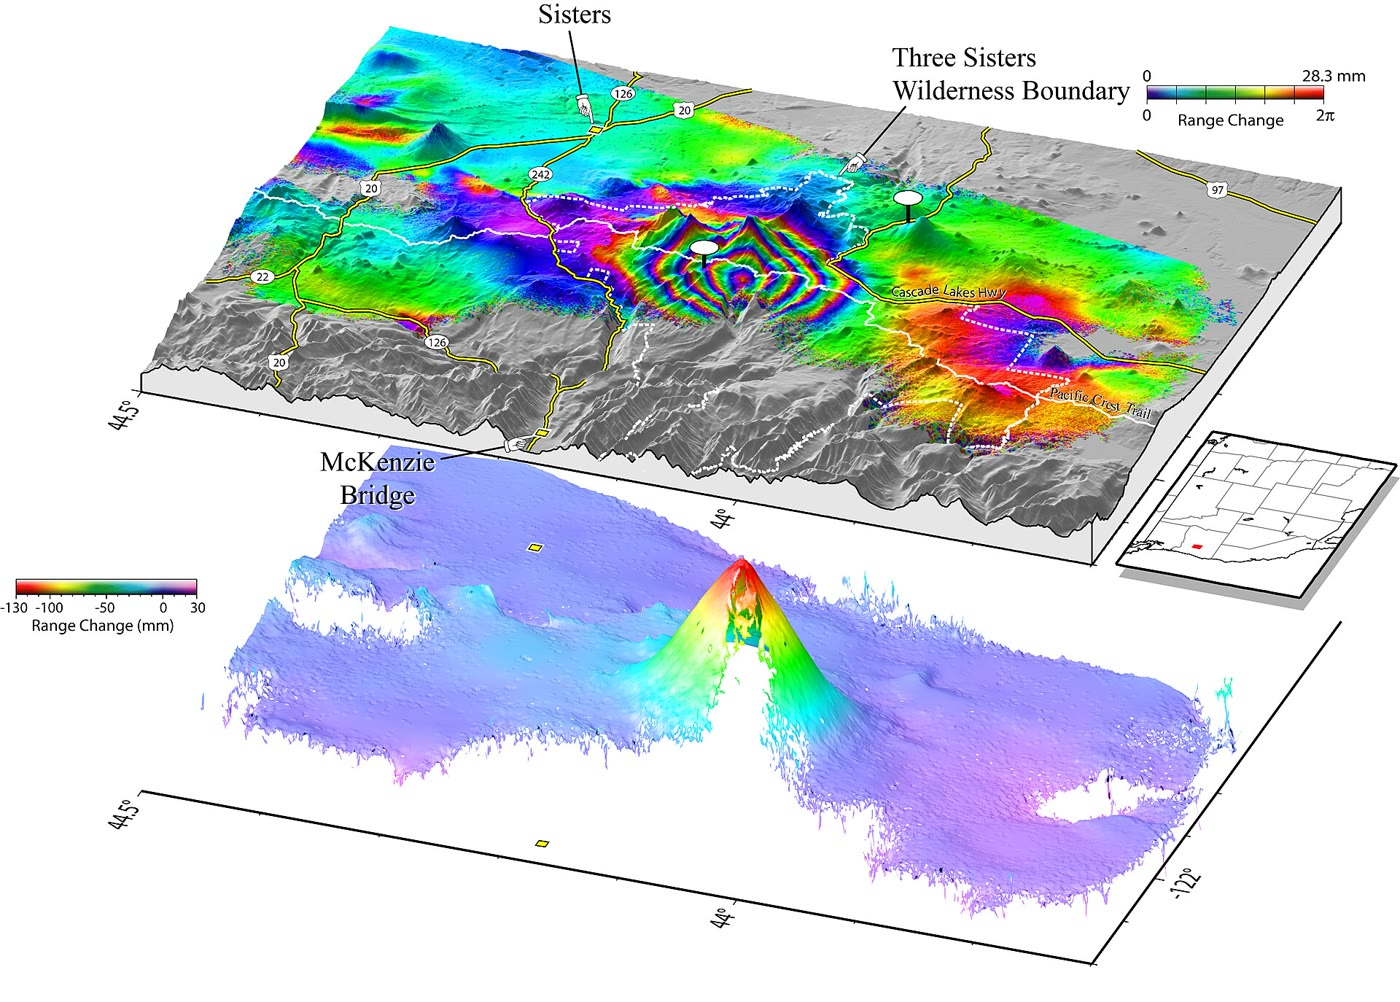
\includegraphics[width=0.86\linewidth]{images/book5/b3-three-sisters-insar.jpg}
\par\smallskip{\small Above, the \omterm{def:b3:remote-sensing-gis:insar}{interferogram} of the Three Sisters
volcanic centre, Oregon, 1995--2001, draped over the relief: each cycle of
colours is \qty{28.3}{mm} of range change, and the bull's eye of rings at
the centre marks the uplift. Below, the same data unwrapped and drawn as a
relief: the range shortens by up to \qty{130}{mm} at the centre. U.S.
Geological Survey (Wicks and others, 2002), public
domain.}\label{fig:b3:remote-sensing-gis:three-sisters}
\end{omfigure}
% ledger: photo:b3-three-sisters-insar, usgs:insar-fs

\begin{inthelab}[A ground station]
\begin{minipage}[t]{0.55\linewidth}\vspace{0pt}
An imaging satellite records far more than it can send while it passes
over the place it images. The radar of a Sentinel-1 satellite can image
for up to half an hour of each orbit and stores its data on board, up to
1410 gigabits; it sends them down over two channels of 260 megabits a
second each, so a full store takes some 45 minutes to empty. A ground
station receives them: as the satellite rises above the horizon, the dish
turns to point at it, follows it across the sky and lets it go as it sets,
while the operators check that the stream arrives complete. The data then
go to a processing centre, where the raw echoes become images.
\end{minipage}\hfill
\begin{minipage}[t]{0.42\linewidth}\vspace{0pt}
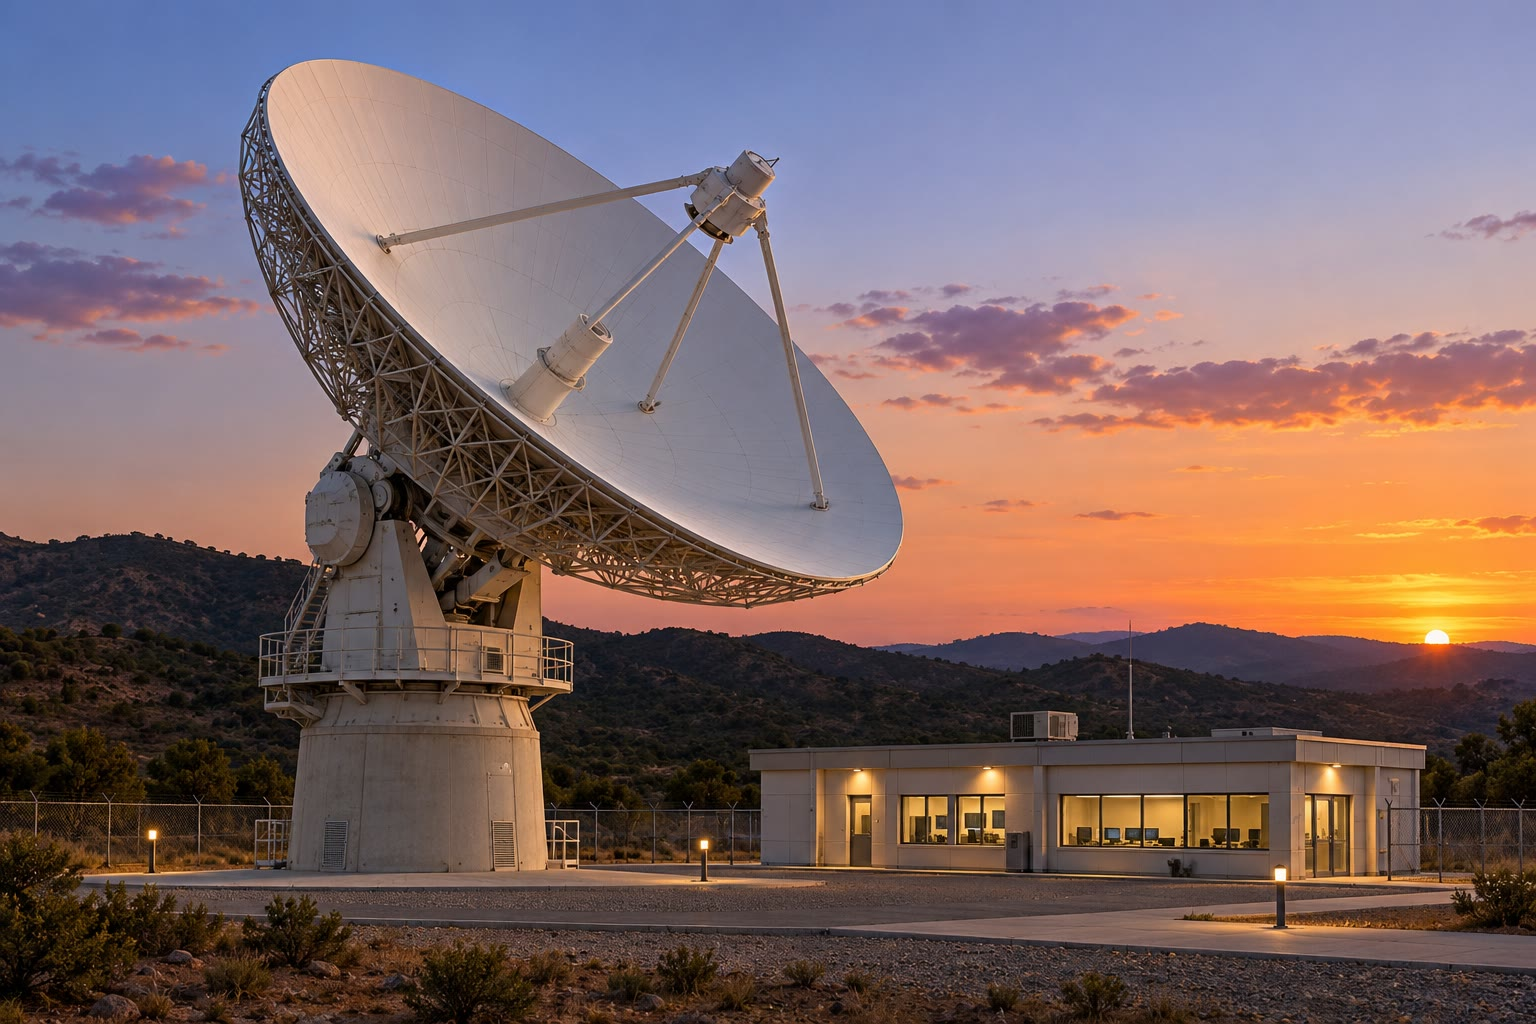
\includegraphics[width=\linewidth]{images/book5/ai/b3-ground-station.jpg}

{\scriptsize A satellite ground station at dusk: a large tracking dish and
its operations building (AI-generated illustration).}
\end{minipage}
\end{inthelab}
% ledger: esa:s1-downlink

\section{Geographic information systems}\label{sec:b3:remote-sensing-gis:gis}

The images of the satellites, the elevation model of the ground, the
geological map, the wells and the roads are layers of one geographic
information system, which stores them in a common frame of coordinates and
computes with them.

\begin{definition}[Raster and vector data]\label{def:b3:remote-sensing-gis:data-models}
\emph{Raster data}\index{raster data} represent a layer by a grid of
cells, each holding one value: a reflectance, an elevation, a class.
\emph{Vector data}\index{vector data (GIS)} represent it by points, lines
and polygons given by the coordinates of their vertices, each carrying a
row of attributes in a table.
\end{definition}

\begin{omfigure}
\centering
\begin{tikzpicture}[x=0.5cm, y=0.5cm, font=\scriptsize]
\begin{scope}
\draw[black!40] (0,0) rectangle (10,7);
\fill[omSea!50, draw=omDef, thick] (3,4.5) ellipse (1.8 and 1.2);
\draw[omDef, very thick] (4.8,4.5) -- (7,3.5) -- (10,2);
\fill[red!70!black] (7,5.5) circle (0.14); \fill[red!70!black] (2,1.5) circle (0.14);
\node[anchor=south] at (5,7.1) {vector};
\node at (3,4.5) {lake};
\node[anchor=south west] at (7.1,5.6) {well 1};
\node[anchor=south west] at (2.1,1.6) {well 2};
\node[anchor=north east] at (9.9,2.2) {river};
\end{scope}
\begin{scope}[xshift=6.5cm]
\foreach \i/\j in {1/4,2/4,3/4,4/4,2/3,3/3,2/5,3/5} {\fill[omSea!50] (\i,\j) rectangle ++(1,1);}
\foreach \i/\j in {5/4,6/3,7/3,8/2,9/2} {\fill[omDef!70] (\i,\j) rectangle ++(1,1);}
\foreach \i/\j in {7/5,2/1} {\fill[red!70!black] (\i,\j) rectangle ++(1,1);}
\draw[black!30, step=1] (0,0) grid (10,7);
\draw[black!40] (0,0) rectangle (10,7);
\node[anchor=south] at (5,7.1) {raster};
\end{scope}
\end{tikzpicture}
\par\smallskip{\small The same map as vector data (left: a polygon, a line
and two points, exact in position, each with its attributes) and as \omterm{def:b3:remote-sensing-gis:data-models}{raster
data} (right: one value per cell, the lake by the cells whose centre lies in
it, the river and the wells by the cells they cross). A raster is easy to
compute with, cell by cell; a vector layer keeps shapes and topology at
any scale.}\label{fig:b3:remote-sensing-gis:raster-vector}
\end{omfigure}

\begin{definition}[Georeferencing]\label{def:b3:remote-sensing-gis:georef}
\emph{Georeferencing}\index{georeferencing} is the assignment of map
coordinates in a stated projection to every pixel of an image or every
vertex of a drawing, usually by fitting a transformation to ground control
points whose positions are known in both.
\end{definition}

For a north-up raster in a projected frame the transformation is affine:
the cell in column $i$ and row $j$ has its corner at $E = E_0 + i\,\Delta$,
$N = N_0 - j\,\Delta$, with $\Delta$ the cell size. A satellite image is
first resampled into such a grid; layers in different projections are
projected into one before they are combined.

\begin{method}[Slope, aspect and hillshade from a digital elevation model]\label{met:b3:remote-sensing-gis:slope}
On a grid of elevations $z_{i,j}$ of spacing $\Delta$ ($i$ eastward, $j$
northward), estimate the gradient by central differences,
\[
\frac{\partial z}{\partial x} \approx \frac{z_{i+1,j} - z_{i-1,j}}{2\Delta} ,
\qquad
\frac{\partial z}{\partial y} \approx \frac{z_{i,j+1} - z_{i,j-1}}{2\Delta} .
\]
The \emph{slope} is $S = \arctan|\nabla z|$; the \emph{aspect} is the
azimuth of steepest descent, the direction of $-\nabla z$, $A =
\operatorname{atan2}(-\partial z/\partial x, -\partial z/\partial y)$
measured clockwise from north. The \emph{hillshade} for a light from the
azimuth $A_0$ at the zenith angle $Z$ is $\cos Z\cos S + \sin Z\sin S
\cos(A_0 - A)$, the cosine of the angle between the light and the normal
to the ground, set to zero where it is negative.
\end{method}

The central difference is exact for a plane and in error by
$\Delta^2 z'''/6$ otherwise; the shaded relief of the Varden Hills in the
Year~1 volume was computed this way, lit from the north-west. Derivatives
amplify the errors of the grid: a model with steps between its rows shows
them as stripes in its slope map.

\begin{definition}[Map algebra]\label{def:b3:remote-sensing-gis:map-algebra}
\emph{Map algebra}\index{map algebra} is the computation of a new raster
layer cell by cell from one or more layers of the same grid: by arithmetic
(the NDVI from two bands), by comparison (the cells steeper than
\ang{15}), by logical operations (and, or, not), or from a neighbourhood
of the cell (the slope).
\end{definition}

\begin{definition}[Buffer; overlay]\label{def:b3:remote-sensing-gis:operations}
The \emph{buffer}\index{buffer (GIS)} of a feature at the distance $d$ is
the region of the map within $d$ of it. An
\emph{overlay}\index{overlay (GIS)} combines two or more layers of the
same area into one, each place of the result carrying the attributes of
all of them; the selection of the places that meet several conditions at
once is the commonest use.
\end{definition}

\begin{omfigure}
\centering
\begin{tikzpicture}
\begin{groupplot}[group style={group size=2 by 2, horizontal sep=2.0cm, vertical sep=1.5cm},
  width=0.43\linewidth, axis equal image, enlargelimits=false,
  xmin=0, xmax=10, ymin=0, ymax=8,
  tick label style={font=\scriptsize}, label style={font=\small}, title style={font=\small}]
\nextgroupplot[title={(a) slope (degrees)}, ylabel={north (km)}, colormap/viridis,
  point meta min=0, point meta max=24, colorbar right,
  colorbar style={width=0.18cm, ytick={0,5,10,15,20}, tick label style={font=\tiny}, axis equal=false}]
\addplot[matrix plot*, mesh/cols=101, point meta=explicit] table[x=x, y=y, meta=slope] {figdata/out/bachelor-3-varden_gis-grid.dat};
\addplot[white, thick] table {figdata/out/shared-region-river.dat};
\nextgroupplot[title={(b) aspect},
  colormap={aspect}{rgb255=(220,20,30) rgb255=(240,200,0) rgb255=(30,170,60) rgb255=(30,90,220) rgb255=(220,20,30)},
  point meta min=0, point meta max=360, colorbar right,
  colorbar style={width=0.18cm, ytick={0,90,180,270,360}, yticklabels={N,E,S,W,N}, tick label style={font=\tiny}, axis equal=false}]
\addplot[matrix plot*, mesh/cols=101, point meta=explicit] table[x=x, y=y, meta=aspect] {figdata/out/bachelor-3-varden_gis-grid.dat};
\addplot[black, thick] table {figdata/out/shared-region-river.dat};
\nextgroupplot[title={(c) two layers}, xlabel={east (km)}, ylabel={north (km)},
  colormap={lay}{rgb255=(245,245,245) rgb255=(150,150,150) rgb255=(225,195,140) rgb255=(120,70,20)},
  colormap access=piecewise constant, point meta min=-0.5, point meta max=3.5,
  legend columns=2, legend style={font=\tiny, at={(0.5,-0.3)}, anchor=north, /tikz/every even column/.append style={column sep=4pt}}]
\addplot[matrix plot*, mesh/cols=101, point meta=explicit, forget plot] table[x=x, y=y, meta=layers] {figdata/out/bachelor-3-varden_gis-grid.dat};
\addplot[omDef, thick, forget plot] table {figdata/out/shared-region-river.dat};
\addlegendimage{area legend, fill={rgb,255:red,150;green,150;blue,150}, draw=black!40}
\addlegendentry{steeper than \ang{15}}
\addlegendimage{area legend, fill={rgb,255:red,225;green,195;blue,140}, draw=black!40}
\addlegendentry{shale}
\addlegendimage{area legend, fill={rgb,255:red,120;green,70;blue,20}, draw=black!40}
\addlegendentry{both}
\nextgroupplot[title={(d) the overlay}, xlabel={east (km)},
  colormap={cls}{rgb255=(245,245,245) rgb255=(225,195,140) rgb255=(190,150,90) rgb255=(200,20,30)},
  colormap access=piecewise constant, point meta min=-0.5, point meta max=3.5,
  legend columns=2, legend style={font=\tiny, at={(0.5,-0.3)}, anchor=north, /tikz/every even column/.append style={column sep=4pt}}]
\addplot[matrix plot*, mesh/cols=101, point meta=explicit, forget plot] table[x=x, y=y, meta=class] {figdata/out/bachelor-3-varden_gis-grid.dat};
\addplot[omDef, thick, forget plot] table {figdata/out/shared-region-river.dat};
\addplot[black, thin, dashed, unbounded coords=jump] table[x=x, y=y] {figdata/out/bachelor-3-varden_gis-buffer.dat};
\addlegendentry{\qty{1}{km} buffer}
\addlegendimage{area legend, fill={rgb,255:red,225;green,195;blue,140}, draw=black!40}
\addlegendentry{shale}
\addlegendimage{area legend, fill={rgb,255:red,190;green,150;blue,90}, draw=black!40}
\addlegendentry{shale in buffer}
\addlegendimage{area legend, fill={rgb,255:red,200;green,20;blue,30}, draw=black!40}
\addlegendentry{selected}
\end{groupplot}
\end{tikzpicture}
\par\smallskip{\small A GIS session on the Varden Hills, from their elevation
model on a \qty{100}{m} grid. (a)~The slope, up to \ang{23} on the valley
sides; (b)~the aspect, the direction the ground faces, the two sides of the
river facing each other; (c)~two layers, the cells steeper than \ang{15}
and the outcrop of the Jurassic shale; (d)~their \omterm{def:b3:remote-sensing-gis:operations}{overlay} with the
\qty{1}{km} \omterm{def:b3:remote-sensing-gis:operations}{buffer} of the river (dashed): the \qty{0.32}{km^2} of steep
shale above the river, a first screen for ground that may
slide.}\label{fig:b3:remote-sensing-gis:varden}
\end{omfigure}

The figure above runs the whole chain: \omterm{def:b3:remote-sensing-gis:map-algebra}{map algebra} on the elevation grid
gives the slope and the aspect; a comparison turns the slope into a layer
of steep cells; the geological map gives the shale; the \omterm{def:b3:remote-sensing-gis:operations}{buffer} of the
river gives a third layer; their intersection, an \omterm{def:b3:remote-sensing-gis:operations}{overlay} with the logical
\emph{and}, leaves 32 cells of the 8181. The answer is only as good as the
layers: on a coarser grid the slopes come out gentler and fewer cells pass.

\begin{definition}[Supervised classification; confusion matrix]\label{def:b3:remote-sensing-gis:classification}
A \emph{supervised classification}\index{supervised classification}
assigns each pixel of an image to one of a set of classes, from rules or
statistics learned on training pixels whose class is known on the ground.
Its \emph{confusion matrix}\index{confusion matrix} counts, for a separate
set of reference pixels, how many of each true class were assigned to each
class: $n_{ij}$ pixels classified as $i$ belong in truth to $j$.
\end{definition}

The diagonal holds the pixels classified right. With $N$ reference pixels,
the \emph{overall accuracy} is $\sum_i n_{ii}/N$. The \emph{user's
accuracy} of a class, $n_{ii}$ over its row total, is the chance that a
pixel the map calls $i$ is $i$; its \emph{producer's accuracy}, $n_{ii}$
over its column total, the chance that a true $i$ was mapped as $i$. The
\emph{kappa} coefficient compares the overall accuracy $p_o$ with the
accuracy $p_e = \sum_i (\text{row}_i)(\text{col}_i)/N^2$ that random
assignment with the same totals would reach: $\kappa = (p_o - p_e)/(1 -
p_e)$.

\begin{center}
\small
\begin{tabular}{l|ccc|c}
\hline
classified \textbackslash{} reference & water & forest & bare rock & total \\
\hline
water & 45 & 2 & 0 & 47 \\
forest & 3 & 38 & 7 & 48 \\
bare rock & 0 & 5 & 30 & 35 \\
\hline
total & 48 & 45 & 37 & 130 \\
\hline
\end{tabular}
\end{center}

In this invented example, 113 of 130 pixels are right, an overall accuracy
of \qty{86.9}{\percent}. Forest has a user's accuracy of
$38/48 = \qty{79}{\percent}$ but a producer's accuracy of $38/45 =
\qty{84}{\percent}$: seven pixels of bare rock, perhaps in shadow, were
called forest. Random assignment would reach $p_e = 0.338$, and $\kappa =
0.80$.

\section{Exercises}

\begin{exercise}[$\star$]\label{exo:b3:remote-sensing-gis:1}
A field has reflectances of 0.06 in the red band and 0.42 in the
near-infrared band of an imager; a ploughed field next to it 0.21 and
0.28. Compute the NDVI of both and say what each value suggests.
\end{exercise}

\begin{exercise}[$\star$]\label{exo:b3:remote-sensing-gis:2}
The Landsat~8 imager covers a swath \qty{185}{km} wide with \qty{30}{m}
pixels, and its panchromatic band with \qty{15}{m} pixels. (a)~How many
pixels does a line across the swath hold in each case? (b)~How many levels
do 12 bits give, and 8 bits? (c)~What is the \omterm{def:b3:remote-sensing-gis:resolutions}{revisit time} of Landsat~8
alone, and of Landsats 8 and 9 together?
\end{exercise}

\begin{exercise}[$\star$]\label{exo:b3:remote-sensing-gis:3}
(a)~On a Sentinel-1 \omterm{def:b3:remote-sensing-gis:insar}{interferogram} ($\lambda = \qty{5.55}{cm}$) of a
subsiding basin, six fringes separate the stable edge from the centre.
What is the change of the \omterm{def:b3:remote-sensing-gis:insar}{line of sight} at the centre? (b)~What would one
fringe be for an older satellite of wavelength \qty{5.66}{cm}?
\end{exercise}

\begin{exercise}[$\star$]\label{exo:b3:remote-sensing-gis:4}
A laser altimeter is \qty{500}{km} above the ground. (a)~How long does a
pulse take to return? (b)~If each photon is timed to \qty{800}{ps}, how
precise is one range?
\end{exercise}

\begin{exercise}[$\star\star$]\label{exo:b3:remote-sensing-gis:5}
A pixel of Landsat~8's band~10 (take $\lambda = \qty{10.9}{\micro\metre}$)
has, after \omterm{def:b3:remote-sensing-gis:atm-correction}{atmospheric correction}, a spectral radiance of
\qty{9.0}{W.m^{-2}.sr^{-1}.\micro\metre^{-1}}. (a)~Compute its \omterm{def:b3:remote-sensing-gis:brightness}{brightness
temperature}. (b)~The surface is a grass field of emissivity 0.98: what is
its kinetic temperature?
\end{exercise}

\begin{exercise}[$\star\star$]\label{exo:b3:remote-sensing-gis:6}
The Sentinel-1 radar flies \qty{693}{km} up with an antenna \qty{12.3}{m}
long at $\lambda = \qty{5.55}{cm}$. (a)~Ignoring the curvature of the
Earth, compute the slant range to a point seen at an incidence of
\ang{35}. (b)~What azimuth resolution would a real antenna of that length
give there, and what does the synthetic aperture give? (c)~How long is the
synthetic aperture?
\end{exercise}

\begin{exercise}[$\star\star$]\label{exo:b3:remote-sensing-gis:7}
A $3\times3$ window of a digital elevation model with \qty{30}{m} cells
reads, north at the top,
\[
\begin{matrix} 412 & 418 & 425 \\ 405 & 410 & 418 \\ 398 & 401 & 409 \end{matrix}
\qquad (\unit{m}).
\]
By central differences at the centre cell, compute the slope, the aspect
and the hillshade for a light from the north-west, \ang{45} above the
horizon.
\end{exercise}

\begin{exercise}[$\star\star$]\label{exo:b3:remote-sensing-gis:8}
A land-cover map is checked against 160 reference pixels (rows: the map;
columns: the truth; classes water, forest, crops, town):
\[
\begin{pmatrix} 48 & 3 & 1 & 0 \\ 4 & 37 & 6 & 1 \\ 2 & 5 & 29 & 2 \\ 0 & 1 & 2 & 19 \end{pmatrix} .
\]
Compute the overall accuracy, the user's and producer's accuracies of each
class, and kappa. Which class is most often missed?
\end{exercise}

\begin{exercise}[$\star\star$]\label{exo:b3:remote-sensing-gis:9}
A \qty{100}{m} thermal pixel contains a fresh lava flow at \qty{1443}{K}
covering \qty{4}{\percent} of it; the rest is ground at \qty{290}{K}; take
both as black bodies. (a)~Compute the \omterm{def:b3:remote-sensing-gis:brightness}{brightness temperature} of the pixel
at \qty{10.9}{\micro\metre} and compare it with the mean temperature.
(b)~Compute the ratio of the black-body radiances of the lava and the
ground at \qty{2.2}{\micro\metre}, and the \omterm{def:b3:remote-sensing-gis:brightness}{brightness temperature} of the
pixel there. Which band detects the lava better?
\end{exercise}

\begin{exercise}[$\star\star\star$]\label{exo:b3:remote-sensing-gis:10}
Two \omterm{def:b3:remote-sensing-gis:insar}{interferograms} of the same deformation are made from two passes, one
with the satellite to the east of the ground and one with it to the west,
both at an incidence of \ang{35}. At one point the
\omterm{def:b3:remote-sensing-gis:insar}{line of sight} shortens by \qty{64}{mm} on the first and \qty{38}{mm} on
the second. Assuming no north--south motion, compute the vertical and the
eastward displacements. Why is one pass not enough?
\end{exercise}

\begin{exercise}[$\star\star\star$]\label{exo:b3:remote-sensing-gis:11}
Unwrapping fails where the phase jumps by more than $\pi$ between
neighbouring pixels. (a)~Show that the \omterm{def:b3:remote-sensing-gis:insar}{line of sight} must change by less
than $\lambda/4$ from one pixel to the next, \qty{13.9}{mm} for
Sentinel-1. (b)~For a Mogi source at $z_0 = \qty{4}{km}$ with $\Delta V =
\qty{e7}{m^3}$ and $\nu = 0.25$, seen vertically, show that the steepest
gradient of $u_z$ is at $r = z_0/2$ and compute it. (c)~What is the
largest pixel size that keeps the fringes resolvable?
\end{exercise}

\begin{exercise}[$\star\star\star$]\label{exo:b3:remote-sensing-gis:12}
(a)~Show that the NDVI lies between $-1$ and $+1$ for non-negative
reflectances, and that it is unchanged when both reflectances are
multiplied by the same factor. (b)~Grass has reflectances of 0.051 (red)
and 0.502 (near infrared). An uncorrected image adds a path radiance
equivalent to 0.03 in the red and 0.01 in the near infrared. Compute the
NDVI with and without it. (c)~What does that imply for a map of the NDVI
made from uncorrected images on a hazy day?
\end{exercise}

\section{Problem: A Swelling Flank at Mount Halvren}

\begin{problem}[{Weekend problem --- vegetation, heat and a radar
interferogram on an invented volcano}]
\label{pb:b3:remote-sensing-gis:1}
Mount Halvren, an invented volcano, has erupted lava flows in 1890, 1960
and 2005 onto its forested flanks. A fumarole field steams on its summit.
Satellite data of a recent year are given below.

\medskip\noindent\textbf{Part I --- Vegetation on the lava flows.} Corrected
reflectances in the red and near-infrared bands:
\begin{center}
\small
\begin{tabular}{lcccc}
\hline
surface & forest & flow of 1890 & flow of 1960 & flow of 2005 \\
\hline
red & 0.04 & 0.07 & 0.11 & 0.12 \\
near infrared & 0.38 & 0.30 & 0.21 & 0.14 \\
\hline
\end{tabular}
\end{center}
\begin{enumerate}
\item Compute the NDVI of the four surfaces.
\item Rank the flows by the recovery of their vegetation. Is the ranking
  that of their ages?
\item Why is the NDVI of the flow of 2005 not zero, although almost
  nothing grows on it?
\item Why is the NDVI more reliable than the near-infrared reflectance
  alone on the steep, unevenly lit flanks of a volcano?
\end{enumerate}

\medskip\noindent\textbf{Part II --- The fumarole field.} In the thermal
band (take $\lambda = \qty{10.9}{\micro\metre}$) the corrected radiance of
a \qty{100}{m} pixel of the summit plateau away from the fumaroles is
\qty{8.40}{W.m^{-2}.sr^{-1}.\micro\metre^{-1}}, and that of the pixel over
the fumarole field \qty{9.95}{W.m^{-2}.sr^{-1}.\micro\metre^{-1}}.
\begin{enumerate}[resume]
\item Compute the \omterm{def:b3:remote-sensing-gis:brightness}{brightness temperatures} of the two pixels.
\item The plateau's rock has an emissivity of 0.97. What is its kinetic
  temperature?
\item The fumarole vents and the warm ground around them are at
  \qty{370}{K}. Treating them and the rest of the pixel as black bodies,
  the rest at the plateau's radiance, what fraction of the pixel do they
  cover, and what area?
\item Why does the area-weighted mean temperature of the pixel fall short
  of its \omterm{def:b3:remote-sensing-gis:brightness}{brightness temperature}?
\end{enumerate}

\medskip\noindent\textbf{Part III --- The interferogram.} Two Sentinel-1
images ($\lambda = \qty{5.55}{cm}$, incidence \ang{35}, satellite to the
east) taken 48 days apart show a bull's eye on the east flank. From a
stable area to the centre of the pattern one counts five full fringes and
four tenths of a sixth, all of them in the sense of motion towards the
satellite.
\begin{enumerate}[resume]
\item Why must two images be taken from nearly the same position, and how
  many orbital cycles of one satellite separate them?
\item Compute the change of the \omterm{def:b3:remote-sensing-gis:insar}{line of sight} at the centre.
\item At the centre the ground moves only vertically. Compute the uplift
  there.
\item Explain why the pattern is not circular, and on which side, east or
  west, the fringes are crowded.
\item Along the north--south line through the centre, the change of the
  \omterm{def:b3:remote-sensing-gis:insar}{line of sight} falls to half its central value \qty{3.4}{km} from the
  centre. Why use that line, and what depth does it give for a Mogi
  source?
\item How many fringes separate the centre from that half-height point?
\item Water vapour in the air can delay the radar waves differently on the
  two dates and draw fringes of its own. How would a second \omterm{def:b3:remote-sensing-gis:insar}{interferogram},
  of another pair of dates, help tell the two apart?
\end{enumerate}

\medskip\noindent\textbf{Part IV --- The volume.} Take $\nu = 0.25$.
\begin{enumerate}[resume]
\item From $u_z(0) = (1 - \nu)\Delta V/(\pi z_0^2)$, compute the volume
  change of the source.
\item Express it as an average rate per day and per year over the 48 days.
\item Compute the largest horizontal displacement and where it occurs.
\item If the reservoir were a sphere of radius $z_0/3$, how large would its
  volume be, and what fraction of it does the change represent?
\item The finite size of a sphere of radius $z_0/3$ changes the uplift by
  about \qty{3}{\percent}. Does it change the answer of question~16
  appreciably, given the precision of the fringe count?
\item What other observation, from Parts I and II or from the ground,
  would support the interpretation of a filling reservoir?
\item Give the volume change of the reservoir under Mount Halvren, in
  millions of cubic metres, to two significant figures.
\end{enumerate}
\end{problem}
% ledger: nasa:ndvi, esa:s1-sar, esa:s1-orbit, esa:s1-iw, dmodels:mogi, dmodels:mogi-radial, const:h, const:c, const:kB
